\begin{problem}[10.]
    $r = \frac{3}{2 + \sin(\theta)}$
\end{problem}

\begin{solution}
    Let's rewrite this badboy first and foremost.
    
    \[r = \frac{\frac{3}{2}} {1 + \frac{1}{2} \cdot \sin(\theta)}\]
    
    $e < 0$ here, which means we have an ellipse. Based on our above theorem, the directrix will be at $y = d$, and with $d = 3$ being the case here our directrix is at $y = 3$. Now we can calculate our major and minor axes.
    
    Major Axis: 
    \begin{align}
        \text{major} &= \frac{2 \cdot e \cdot d}{1 - e^2} \\
        \text{major} &= \frac{2 \cdot \frac{1}{2} \cdot 3}{1 - \left( \frac{1}{2} \right)^2} \\
        \text{major} &= 4
    \end{align}
    
    Minor Axis:
    \begin{align}
        \text{minor} &= \frac{2 \cdot e \cdot d}{\sqrt{1 - e^2}} \\ 
        \text{minor} &= \frac{3}{\frac{\sqrt{3}}{2}} \\
        \text{minor} &\approx 3.46
    \end{align}
    
    Now to calculate our various vertices and co-vertices using $r(\theta)$.
    
    \[r(0) = \frac{3}{2 + 0}\]
    \[r(0) = \frac{3}{2}\]
    This corresponds to horizontal location. So we get $\left( \frac{3}{2} , 0 \right)$
    
    \[r\left( \frac{\pi}{2} \right) = \frac{3}{2 + 0}\]
    \[r(0) = \frac{3}{2}\]
    This corresponds to horizontal location but negative. So we get $\left( -\frac{3}{2} , 0 \right)$
    
    \[r(\pi) = \frac{3}{2 + 1}\]
    \[r(\pi) = 1\]
    This corresponds to vertical location. So we get $\left( 0 , 1 \right)$
    
    \[r\left( \frac{3\pi}{2} \right) = \frac{3}{2 - 1}\]
    \[r\left( \frac{3\pi}{2} \right) = 3\]
    This corresponds to vertical location but negative. So we get $\left( 0 , -3 \right)$
    
    Now we have all of the information we need to plot this one. 
    
    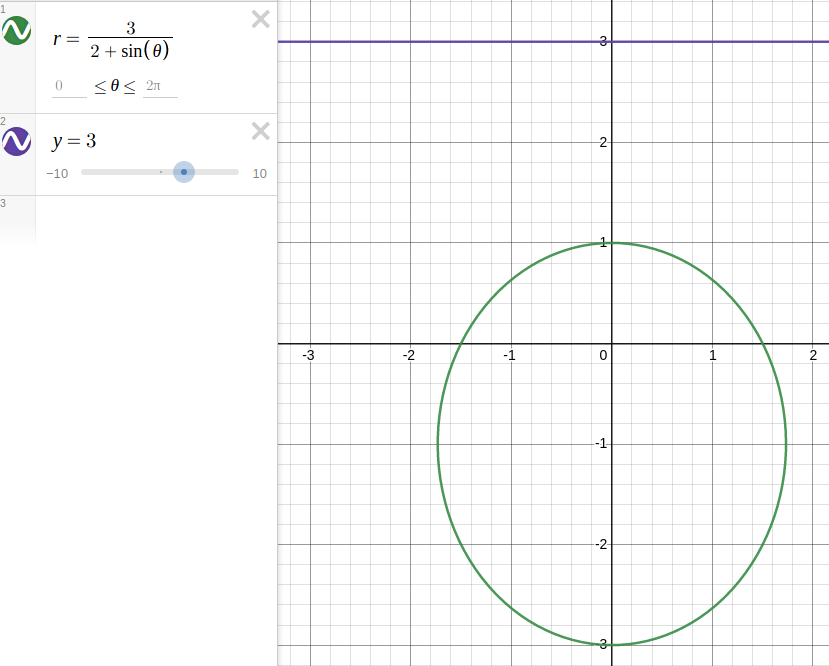
\includegraphics[scale=0.4]{images/11.6_pr_10.png}
\end{solution}